% Options for packages loaded elsewhere
\PassOptionsToPackage{unicode}{hyperref}
\PassOptionsToPackage{hyphens}{url}
\PassOptionsToPackage{dvipsnames,svgnames,x11names}{xcolor}
%
\documentclass[
  letterpaper,
  DIV=11,
  numbers=noendperiod]{scrartcl}

\usepackage{amsmath,amssymb}
\usepackage{lmodern}
\usepackage{iftex}
\ifPDFTeX
  \usepackage[T1]{fontenc}
  \usepackage[utf8]{inputenc}
  \usepackage{textcomp} % provide euro and other symbols
\else % if luatex or xetex
  \usepackage{unicode-math}
  \defaultfontfeatures{Scale=MatchLowercase}
  \defaultfontfeatures[\rmfamily]{Ligatures=TeX,Scale=1}
\fi
% Use upquote if available, for straight quotes in verbatim environments
\IfFileExists{upquote.sty}{\usepackage{upquote}}{}
\IfFileExists{microtype.sty}{% use microtype if available
  \usepackage[]{microtype}
  \UseMicrotypeSet[protrusion]{basicmath} % disable protrusion for tt fonts
}{}
\makeatletter
\@ifundefined{KOMAClassName}{% if non-KOMA class
  \IfFileExists{parskip.sty}{%
    \usepackage{parskip}
  }{% else
    \setlength{\parindent}{0pt}
    \setlength{\parskip}{6pt plus 2pt minus 1pt}}
}{% if KOMA class
  \KOMAoptions{parskip=half}}
\makeatother
\usepackage{xcolor}
\setlength{\emergencystretch}{3em} % prevent overfull lines
\setcounter{secnumdepth}{5}
% Make \paragraph and \subparagraph free-standing
\ifx\paragraph\undefined\else
  \let\oldparagraph\paragraph
  \renewcommand{\paragraph}[1]{\oldparagraph{#1}\mbox{}}
\fi
\ifx\subparagraph\undefined\else
  \let\oldsubparagraph\subparagraph
  \renewcommand{\subparagraph}[1]{\oldsubparagraph{#1}\mbox{}}
\fi


\providecommand{\tightlist}{%
  \setlength{\itemsep}{0pt}\setlength{\parskip}{0pt}}\usepackage{longtable,booktabs,array}
\usepackage{calc} % for calculating minipage widths
% Correct order of tables after \paragraph or \subparagraph
\usepackage{etoolbox}
\makeatletter
\patchcmd\longtable{\par}{\if@noskipsec\mbox{}\fi\par}{}{}
\makeatother
% Allow footnotes in longtable head/foot
\IfFileExists{footnotehyper.sty}{\usepackage{footnotehyper}}{\usepackage{footnote}}
\makesavenoteenv{longtable}
\usepackage{graphicx}
\makeatletter
\def\maxwidth{\ifdim\Gin@nat@width>\linewidth\linewidth\else\Gin@nat@width\fi}
\def\maxheight{\ifdim\Gin@nat@height>\textheight\textheight\else\Gin@nat@height\fi}
\makeatother
% Scale images if necessary, so that they will not overflow the page
% margins by default, and it is still possible to overwrite the defaults
% using explicit options in \includegraphics[width, height, ...]{}
\setkeys{Gin}{width=\maxwidth,height=\maxheight,keepaspectratio}
% Set default figure placement to htbp
\makeatletter
\def\fps@figure{htbp}
\makeatother

\usepackage{booktabs}
\usepackage{longtable}
\usepackage{array}
\usepackage{multirow}
\usepackage{wrapfig}
\usepackage{float}
\usepackage{colortbl}
\usepackage{pdflscape}
\usepackage{tabu}
\usepackage{threeparttable}
\usepackage{threeparttablex}
\usepackage[normalem]{ulem}
\usepackage{makecell}
\usepackage{xcolor}
\KOMAoption{captions}{tableheading}
\makeatletter
\makeatother
\makeatletter
\makeatother
\makeatletter
\@ifpackageloaded{caption}{}{\usepackage{caption}}
\AtBeginDocument{%
\ifdefined\contentsname
  \renewcommand*\contentsname{Table of contents}
\else
  \newcommand\contentsname{Table of contents}
\fi
\ifdefined\listfigurename
  \renewcommand*\listfigurename{List of Figures}
\else
  \newcommand\listfigurename{List of Figures}
\fi
\ifdefined\listtablename
  \renewcommand*\listtablename{List of Tables}
\else
  \newcommand\listtablename{List of Tables}
\fi
\ifdefined\figurename
  \renewcommand*\figurename{Figure}
\else
  \newcommand\figurename{Figure}
\fi
\ifdefined\tablename
  \renewcommand*\tablename{Table}
\else
  \newcommand\tablename{Table}
\fi
}
\@ifpackageloaded{float}{}{\usepackage{float}}
\floatstyle{ruled}
\@ifundefined{c@chapter}{\newfloat{codelisting}{h}{lop}}{\newfloat{codelisting}{h}{lop}[chapter]}
\floatname{codelisting}{Listing}
\newcommand*\listoflistings{\listof{codelisting}{List of Listings}}
\makeatother
\makeatletter
\@ifpackageloaded{caption}{}{\usepackage{caption}}
\@ifpackageloaded{subcaption}{}{\usepackage{subcaption}}
\makeatother
\makeatletter
\@ifpackageloaded{tcolorbox}{}{\usepackage[many]{tcolorbox}}
\makeatother
\makeatletter
\@ifundefined{shadecolor}{\definecolor{shadecolor}{rgb}{.97, .97, .97}}
\makeatother
\makeatletter
\makeatother
\ifLuaTeX
  \usepackage{selnolig}  % disable illegal ligatures
\fi
\IfFileExists{bookmark.sty}{\usepackage{bookmark}}{\usepackage{hyperref}}
\IfFileExists{xurl.sty}{\usepackage{xurl}}{} % add URL line breaks if available
\urlstyle{same} % disable monospaced font for URLs
\hypersetup{
  pdftitle={My title},
  pdfauthor={Sakura Ariga; Aliyah Maxine Ramos; Annie Yan},
  colorlinks=true,
  linkcolor={blue},
  filecolor={Maroon},
  citecolor={Blue},
  urlcolor={Blue},
  pdfcreator={LaTeX via pandoc}}

\title{My title\thanks{Code and data are available at:
https://github.com/AnnieYan0807/GSS-data-analysis.git.}}
\usepackage{etoolbox}
\makeatletter
\providecommand{\subtitle}[1]{% add subtitle to \maketitle
  \apptocmd{\@title}{\par {\large #1 \par}}{}{}
}
\makeatother
\subtitle{My subtitle if needed}
\author{Sakura Ariga \and Aliyah Maxine Ramos \and Annie Yan}
\date{15 March 2023}

\begin{document}
\maketitle
\begin{abstract}
First sentence. Second sentence. Third sentence. Fourth sentence.
\end{abstract}
\ifdefined\Shaded\renewenvironment{Shaded}{\begin{tcolorbox}[interior hidden, breakable, borderline west={3pt}{0pt}{shadecolor}, sharp corners, frame hidden, boxrule=0pt, enhanced]}{\end{tcolorbox}}\fi

\hypertarget{introduction}{%
\section{1 Introduction}\label{introduction}}

You can and should cross-reference sections and sub-sections. For
instance, Section~\ref{sec-data} and Section~\ref{sec-first-point}.

\hypertarget{sec-data}{%
\section{2 Data}\label{sec-data}}

\hypertarget{survey}{%
\subsection{2.1 Survey}\label{survey}}

Saku

\hypertarget{key-features}{%
\subsubsection{2.1.1 Key Features}\label{key-features}}

Saku

\hypertarget{methodology}{%
\subsubsection{2.1.2 Methodology}\label{methodology}}

Saku

\hypertarget{strengths-weaknesses}{%
\subsubsection{2.1.3 Strengths \&
Weaknesses}\label{strengths-weaknesses}}

Saku

\hypertarget{questionnaire}{%
\subsection{2.2 Questionnaire}\label{questionnaire}}

Saku

\hypertarget{overview-of-data}{%
\subsection{2.3 Overview of Data}\label{overview-of-data}}

\hypertarget{data-source}{%
\subsubsection{2.3.1 Data Source}\label{data-source}}

Max

\hypertarget{variables-of-interest}{%
\subsubsection{2.3.2 Variables of
Interest}\label{variables-of-interest}}

Max

\begin{table}

\caption{A subset of key features}
\centering
\begin{tabu} to \linewidth {>{\raggedright}X>{\raggedright}X>{\raggedright}X>{\raggedright}X>{\raggedright}X>{\raggedright}X>{\raggedright}X>{\raggedleft}X}
\hline
Age & Sex & Race & Highest Degree & Number of Children & Marital Status & Happiness Level & Weekly Internet Hours\\
\hline
Ages 40 - 49 & Male & White & Bachelor's & 3 & Married & Pretty happy & 15\\
Ages 60 - 69 & Male & White & High school & 0 & Never married & Pretty happy & 5\\
Ages 70 - 79 & Male & White & Bachelor's & 2 & Married & Very happy & NA\\
Ages 40 - 49 & Female & White & High school & 4 & Married & Pretty happy & 7\\
Ages 50 - 59 & Female & White & Graduate & 2 & Married & Very happy & NA\\
Ages 50 - 59 & Female & White & Associate/junior college & 2 & Married & Very happy & 2\\
Ages 50 - 59 & Male & White & High school & 2 & Married & Pretty happy & 5\\
Ages 21 - 29 & Female & Other & High school & 3 & Married & Very happy & NA\\
\hline
\end{tabu}
\end{table}

Table :)

\begin{figure}

\begin{minipage}[t]{0.50\linewidth}

{\centering 

\raisebox{-\height}{

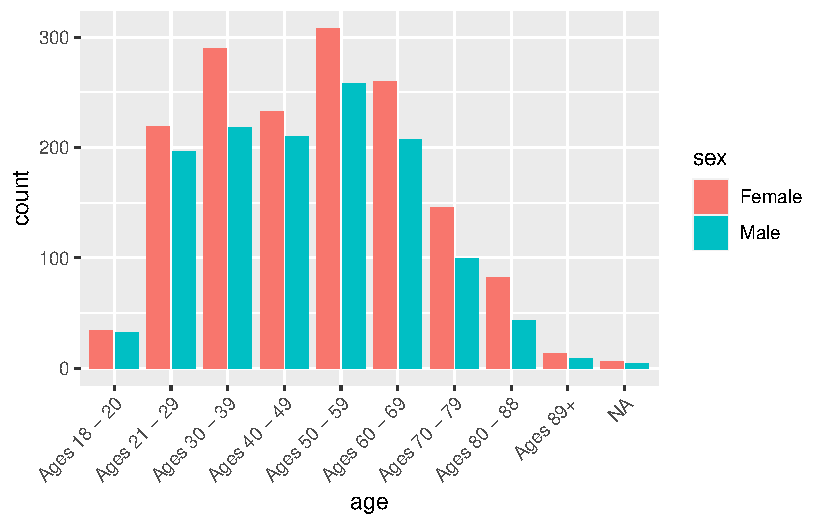
\includegraphics{paper_files/figure-pdf/fig-agesidebyside-1.pdf}

}

}

\subcaption{\label{fig-agesidebyside-1}Subcaption}
\end{minipage}%
%
\begin{minipage}[t]{0.50\linewidth}

{\centering 

\raisebox{-\height}{

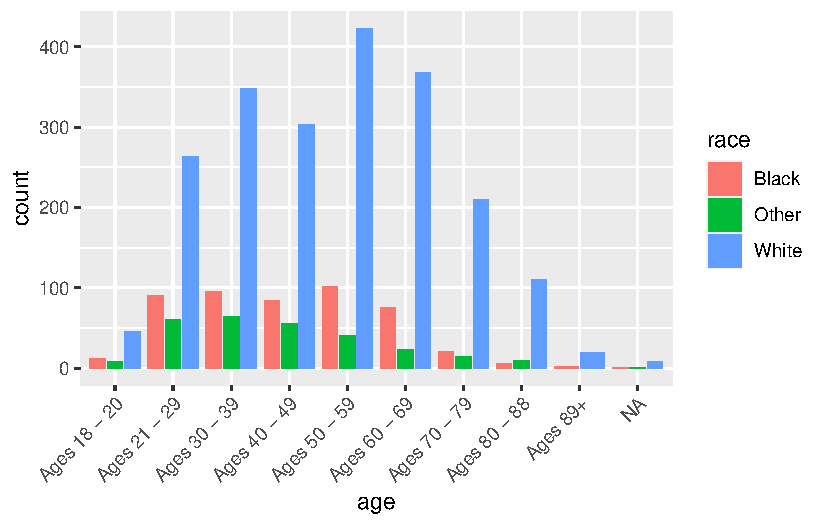
\includegraphics{paper_files/figure-pdf/fig-agesidebyside-2.pdf}

}

}

\subcaption{\label{fig-agesidebyside-2}Subcaption}
\end{minipage}%

\caption{\label{fig-agesidebyside}Caption}

\end{figure}

Figure~\ref{fig-agesidebyside}

\begin{figure}

{\centering 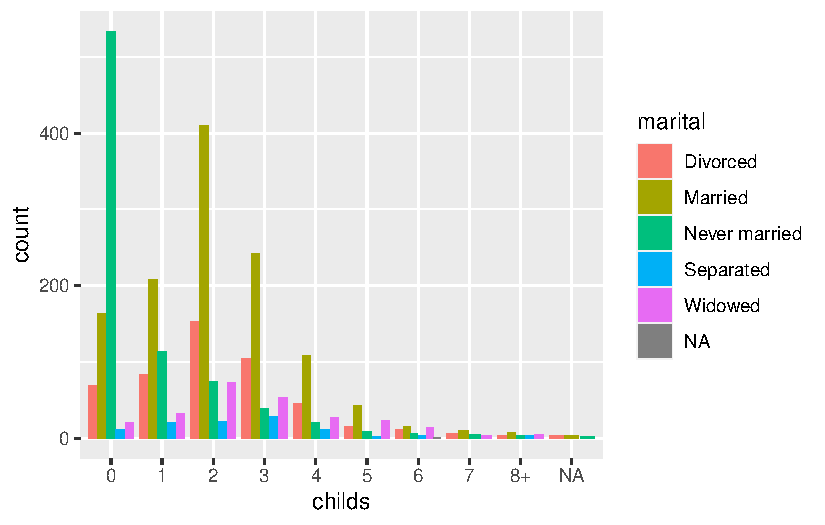
\includegraphics{paper_files/figure-pdf/fig-childsandmarital-1.pdf}

}

\caption{\label{fig-childsandmarital}Caption}

\end{figure}

Figure~\ref{fig-childsandmarital}

\begin{figure}

{\centering 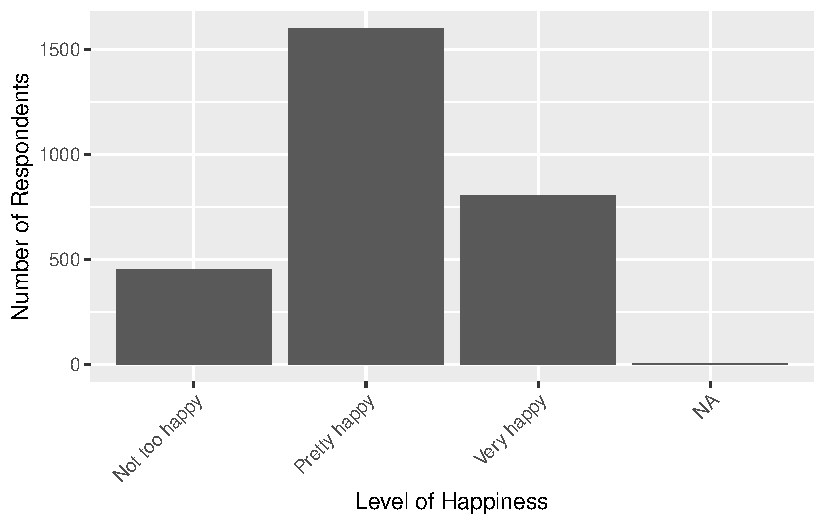
\includegraphics{paper_files/figure-pdf/fig-happiness-1.pdf}

}

\caption{\label{fig-happiness}Caption}

\end{figure}

Figure~\ref{fig-happiness}

\hypertarget{results}{%
\section{3 Results}\label{results}}

\begin{figure}

{\centering 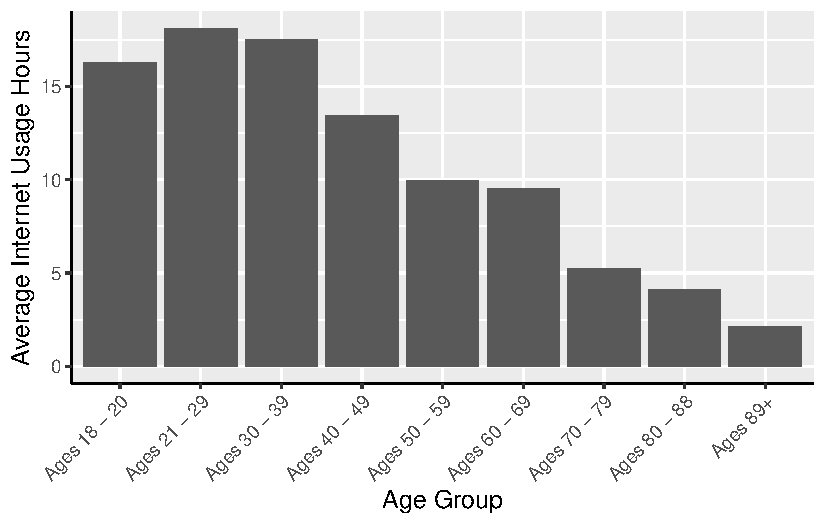
\includegraphics{paper_files/figure-pdf/fig-ageandinternet-1.pdf}

}

\caption{\label{fig-ageandinternet}Average Weekly Total of Internet Use
by Age Group}

\end{figure}

Figure~\ref{fig-ageandinternet} depicting the relationship between age
and average weekly internet usage. The data on internet usage hours for
various age groups are averaged to reduce any bias due to selectively
chosen survey responses. The curve on the graph is skewed to the right,
with its peak occurring in the 21 to 29 age group, which has the highest
internet usage of approximately 18 hours per week. Subsequently,
internet usage gradually declines with age, with the lowest usage
recorded in the 89+ age group at an average of 2 hours per week. This
graph indicates that young adults, particularly those aged 21 to 29,
spend more time on the internet. As people age, their internet usage
tends to decline gradually. The graph suggests a statistically
significant correlation between age and internet usage, and the trend is
relatively clear.

\begin{figure}

{\centering 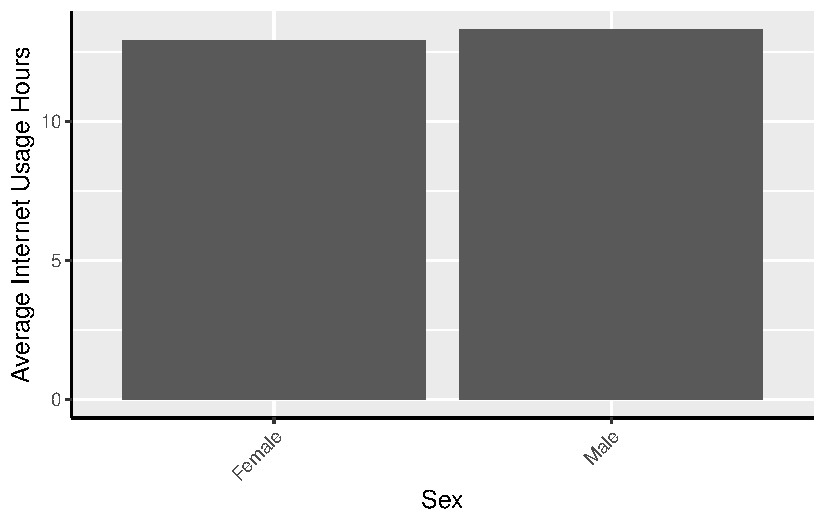
\includegraphics{paper_files/figure-pdf/fig-genderandinternet-1.pdf}

}

\caption{\label{fig-genderandinternet}Average Weekly Total of Internet
Use by Gender}

\end{figure}

Figure~\ref{fig-genderandinternet} illustrates the average weekly
internet usage of two genders. Similarly to the age and internet usage
graph, the data on internet usage hours for different genders are
averaged to minimize any volunteering bias. The data shows that there is
no substantial difference between male and female internet usage. Female
participants have an average of 12.9 hours per week spent on the
internet, while male participants have an slightly higher average of
13.3 hours per week spent on the internet. However, the gender selection
in this survey is limited, and further discussion regarding this
limitation can be found in the ethics and bias section
Section~\ref{sec-bias}.

\begin{figure}

{\centering 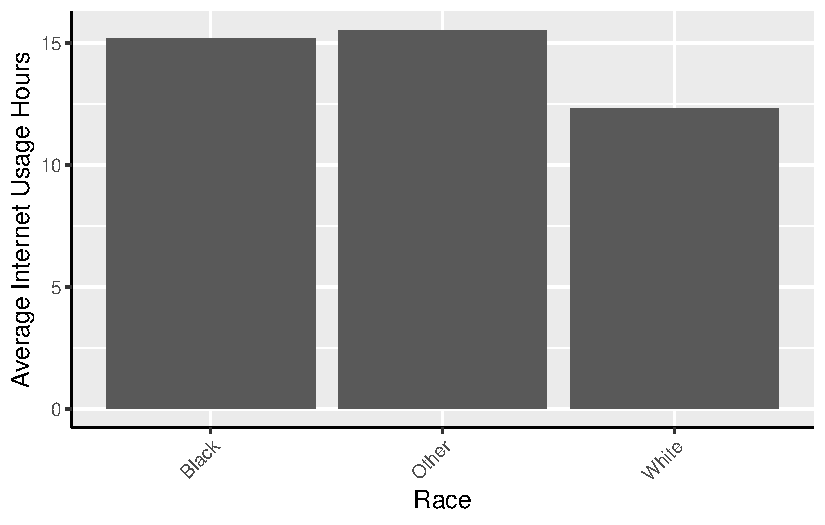
\includegraphics{paper_files/figure-pdf/fig-raceandinternet-1.pdf}

}

\caption{\label{fig-raceandinternet}Average Weekly Total of Internet Use
by Race}

\end{figure}

Figure~\ref{fig-raceandinternet} displays the average weekly internet
usage of individuals belonging to different races. Based on the data, we
can observe that individuals who do not identify as either Black or
White have the highest internet usage, with an average of 15.5 hours per
week. African American individuals have a similar level of internet
usage, also averaging 15.2 hours per week. In contrast, white
individuals tend to have the lowest internet usage, with an average of
12.3 hours per week.

\begin{figure}

{\centering 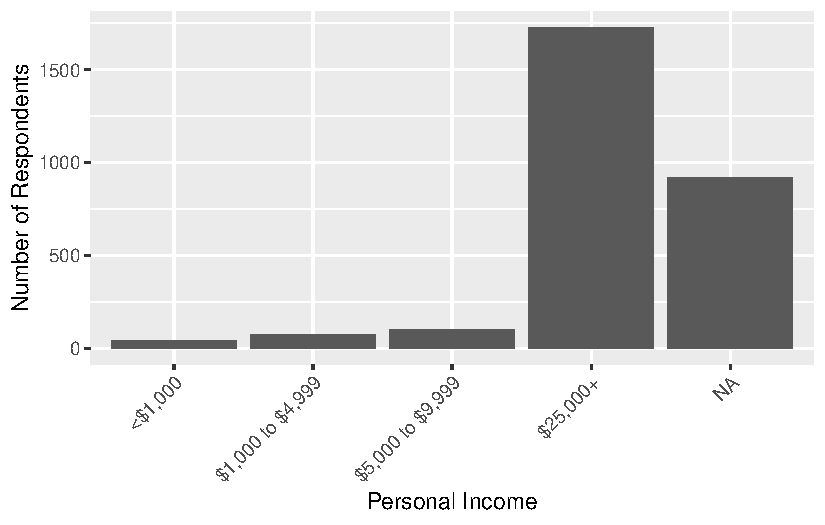
\includegraphics{paper_files/figure-pdf/fig-personalincomeandinternet-1.pdf}

}

\caption{\label{fig-personalincomeandinternet}Average Weekly Total of
Internet Use by Personal Income}

\end{figure}

Max - might emit\ldots{}

\begin{figure}

{\centering 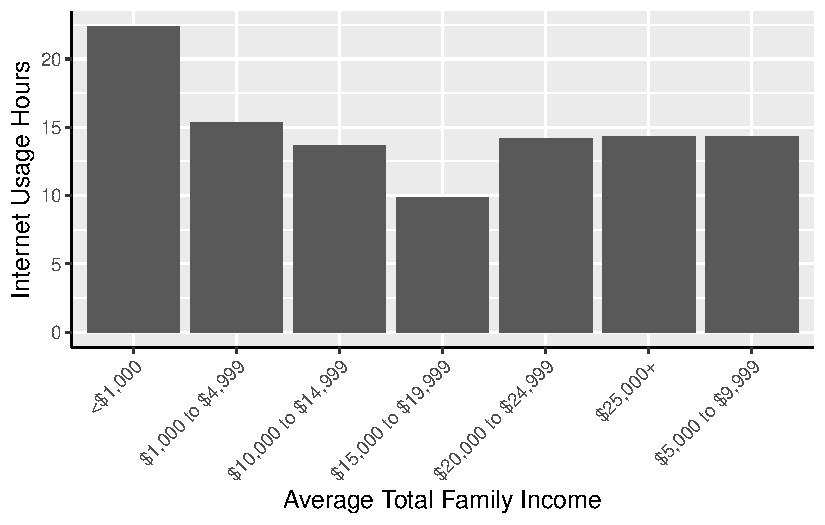
\includegraphics{paper_files/figure-pdf/fig-familyincomeandinternet-1.pdf}

}

\caption{\label{fig-familyincomeandinternet-1}Average Weekly Total of
Internet Use by Family Income}

\end{figure}

\begin{figure}

{\centering 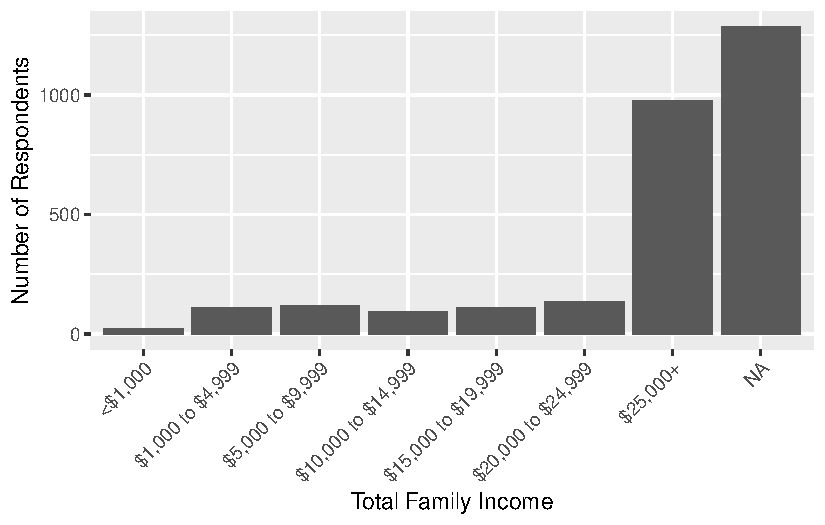
\includegraphics{paper_files/figure-pdf/fig-familyincomeandinternet-2.pdf}

}

\caption{\label{fig-familyincomeandinternet-2}Average Weekly Total of
Internet Use by Family Income}

\end{figure}

Max - might emit

\begin{figure}

{\centering 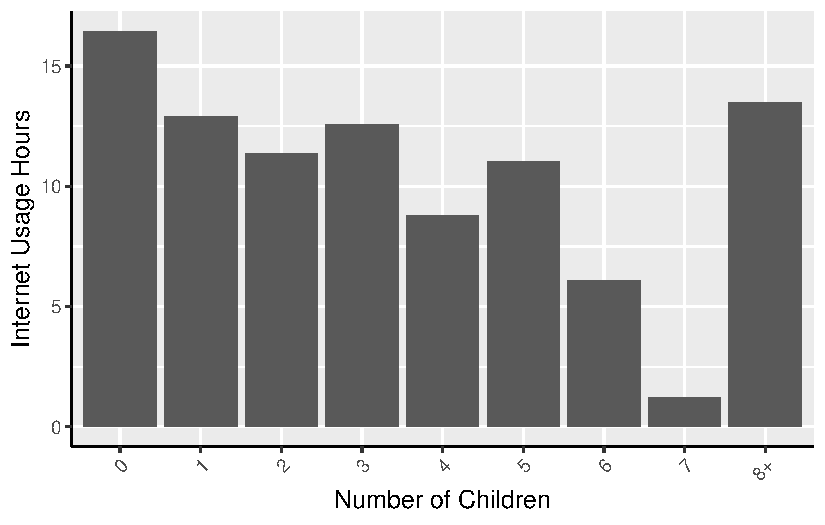
\includegraphics{paper_files/figure-pdf/fig-childrenandinternet-1.pdf}

}

\caption{\label{fig-childrenandinternet}Average Weekly Total of Internet
Use by Children}

\end{figure}

Max

\begin{figure}

{\centering 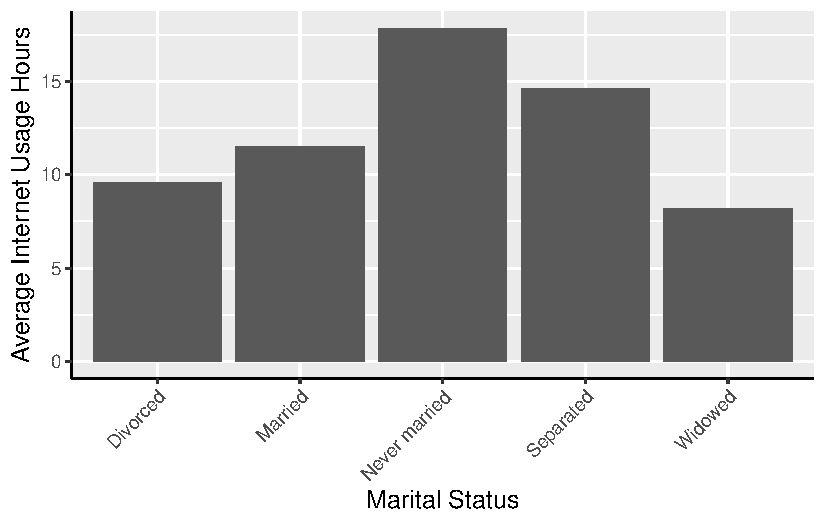
\includegraphics{paper_files/figure-pdf/fig-maritalandinternet-1.pdf}

}

\caption{\label{fig-maritalandinternet}Average Weekly Total of Internet
Use by Marital Status}

\end{figure}

Figure~\ref{fig-maritalandinternet} displays the relationship between
marital status and internet usage in 2016. In accordance with popular
opinion, people who have never been married use the Internet the most.
Most notably, people who are widowed use the Internet the least, perhaps
due to the correlation between age and widowhood.

\begin{figure}

{\centering 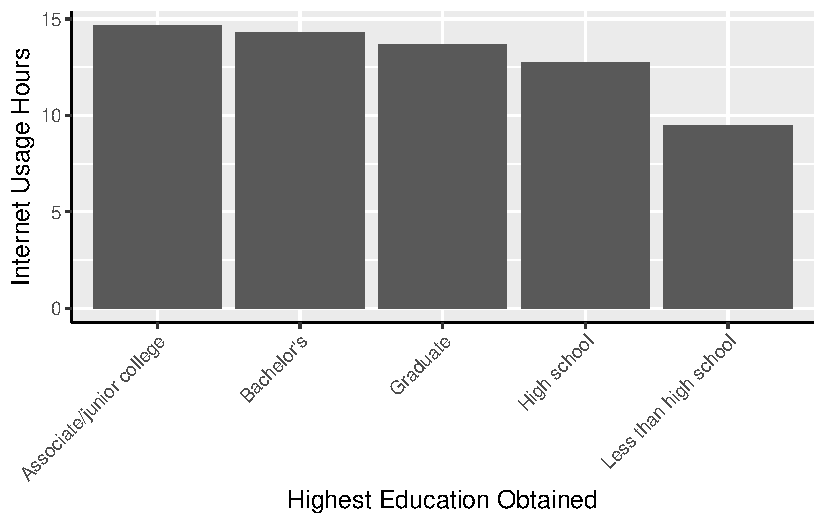
\includegraphics{paper_files/figure-pdf/fig-degreeandinternet-1.pdf}

}

\caption{\label{fig-degreeandinternet}Weekly Total of Internet Use by
Highest Education Obtained}

\end{figure}

Figure~\ref{fig-degreeandinternet} displays the relationship between
highest level of education obtained by the respondent and internet usage
in 2016. Those who have completed a less than high school degree use the
internet the least.

\begin{figure}

{\centering 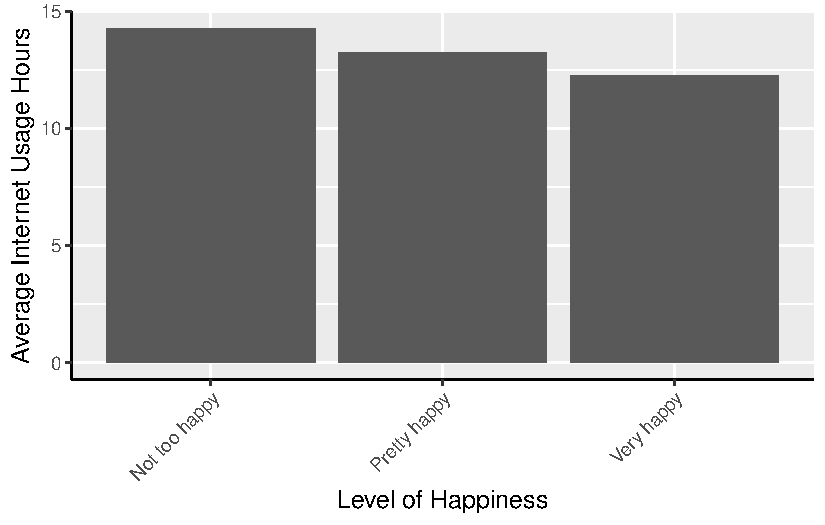
\includegraphics{paper_files/figure-pdf/fig-happyandinternet-1.pdf}

}

\caption{\label{fig-happyandinternet}Average Weekly Total of Internet
Use by Level of Happiness}

\end{figure}

Figure~\ref{fig-happyandinternet} displays the relationship between
perceived level of happiness and internet usage in 2016. There seems to
be a direct decrease in internet usage the more happy the respondent
measures themselves to be, with a difference of 2.5 hours between the
happiest respondents and least happy respondents.

\hypertarget{sec-discussion}{%
\section{4 Discussion}\label{sec-discussion}}

\hypertarget{sec-first-point}{%
\subsection{4.1 First discussion point}\label{sec-first-point}}

\hypertarget{sec-second-point}{%
\subsection{4.2 Second discussion point}\label{sec-second-point}}

\hypertarget{sec-third-point}{%
\subsection{4.3 Third discussion point}\label{sec-third-point}}

\hypertarget{sec-weaknesses}{%
\subsection{4.4 Weaknesses and next steps}\label{sec-weaknesses}}

\hypertarget{sec-bias}{%
\subsection{4.5 Ethics and Bias}\label{sec-bias}}

Based on the data collection methodology provided by GSS, we have
identified some potential biases that could arise. The survey's target
population consists of adults aged 18 and above who reside in households
in the United States. Since this sampling approach focuses only on a
specific age group, our analysis may be biased with respect to the age
factor. Gss also claimed to be strictly voluntary. While this approach
supports research ethics by respecting individuals' autonomy and right
to privacy, it can also result in volunteer bias. GSS sample are from a
mix of urban, suburban, and rural geographic areas, but only a few
thousand respondents are interviewed in the main study. The small sample
size may be lead to chance findings. It is likely not statistically
significant enough. We also suspect potential sampling bias may screw
our end result. However, with not enough information disclosed, we are
unable to confirm that. The gender and race options provided by the GSS
survey are limited. Participants are only given the options of selecting
either ``Female'' or ``Male'' for gender, and ``Blacks,'' ``Whites,'' or
``Others'' for race. This narrow selection does not provide an adequate
range of options for survey participants.

\hypertarget{appendix}{%
\section*{5 Appendix}\label{appendix}}
\addcontentsline{toc}{section}{5 Appendix}

\hypertarget{additional-details}{%
\section{6 Additional details}\label{additional-details}}

\hypertarget{references}{%
\section{7 References}\label{references}}



\end{document}
